% Version 2020-12-15
% update – 161114 by Ken Arroyo Ohori: made spacing closer to Word template throughout, put proper quotes everywhere, removed spacing that could cause labels to be wrong, added non-breaking and inter-sentence spacing where applicable, removed explicit newlines
% update – 010819 by Dennis Wittich: made spacing and font size closer to Word template, updated references and refernces style
% update – 042319 by Dennis Wittich: font size of captions set to 'small', first author names are shortened, hyphenation fixed
% update – 010620 by Dennis Wittich: Footnotes alignment set to left
% update - 151220 by Clement Mallet: Template adapted for double blind full paper submissions
% update - 060321 by Christian Heipke: Template refined for double blind full paper submissions
% update - 090921 by Christian Heipke: Template refined for double blind full paper submissions

\documentclass{isprs} % isprs class modified 23-04-2019 (Dennis Wittich)
\usepackage{subfigure}
\usepackage{setspace}
\usepackage{geometry} % added 27-02-2014 Markus Englich
\usepackage{epstopdf}
\usepackage[labelsep=period]{caption}  % added 14-04-2016 Markus Englich - Recommendation by Sebastian Brocks
\usepackage[british]{babel} 
\usepackage[hang]{footmisc}
\def\footnotemargin{1em} % added 08-01-2020 Dennis Wittich
\usepackage{tabularx}

%\usepackage[authoryear]{natbib}
%\def\bibhang{0pt}

\geometry{a4paper, top=25mm, left=20mm, right=20mm, bottom=25mm, headsep=10mm, footskip=12mm} % added 27-02-2014 Markus Englich
%\usepackage{enumitem}

%\usepackage{isprs}
%\usepackage[perpage,para,symbol*]{footmisc}

%\renewcommand*{\thefootnote}{\fnsymbol{footnote}}
\captionsetup{justification=centering,font=normal} % thanks to Niclas Borlin 05-05-2016
\captionsetup[figure]{font=small} % added 23-04-2019 Dennis Wittich
\captionsetup[table]{font=small} % added 23-04-2019 Dennis Wittich

\begin{document}

\title{SERVING GEOSPATIAL DATA USING MODERN AND LEGACY STANDARDS: A CASE STUDY FROM THE URBAN HEALTH DOMAIN}
\date{}


% KAO: Remove extra spacing
% Anonymous submissions, authors' names should not be visible
\author{***** (for review, names must be rendered anonymous)}

% KAO: Remove extra newline
% Anonymous submissions, authors' affiliations should not be visible
\address{**** (for review, affiliations must be rendered anonymous)}

% If the corresponding author is NOT the final author, always add a % space before the subsequent comma, i.e.
% first author name\textsuperscript{a,}\thanks{Corresponding author} , % second author name \textsuperscript{b}, etc.
% thanks to Niclas Borlin 05-05-2016

\icwg{}   %This field is optional.

% KAO: Use times symbol
\abstract{
	The eMOTIONAL Cities project sets out to understand how the natural and built environment can shape the feelings and emotions of those who experience it. It does so with a cross-disciplinary approach which includes urban planners, doctors, psychologists, neuroscientists and engineers. At the core of this research project, lies a Spatial Data Infrastructure (SDI) which assembles datasets that characterise the emotional landscape and built environment, in different cities across Europe and the US. The SDI is a key tool, not only to make the research data available within the project consortium, but also to allow cross-fertilisation with other ongoing projects and later on, to reach a wider public audience.
	For more than twenty years SDIs have adopted the OGC W*s service interfaces, which are based on SOAP, the Simple Object Access Protocol. In recent years a new “family” of APIs has emerged within OGC, which is more aligned with modern web practices. In this project, we set out to leverage the advantages of this new approach, and compiled a stack to implement an SDI based on OGC APIs. However, we realised that we still need to support the legacy standards, either because an OGC API replacement is not mature enough, or there are no implementations available. This has led us to compile another stack based on the legacy standards. In this paper we describe our architecture, along with the challenges that we had to address. Both stacks are based on OSGeo Software, and they are available on GitHub.
	}

\keywords{Geospatial Data, Standards, Interoperability, API, Spatial Data Infrastructure, Urban Health, pygeoapi, Metadata}

\maketitle

%\saythanks % added 28-02-2014 Markus Englich

\section{INTRODUCTION}\label{INTRODUCTION}
 
% KAO: Sloppy spacing ensures non-overfull lines. Can be removed if this is not an issue.
\sloppy

Urban planning and design play an essential role in amplifying or diminishing built environmental threats to health promotion and disease prevention ~\cite{keedwell2017,hackman2019}. However, there is still a lack of good evidence and objective measures on how environmental aspects impact individual behaviour. The eMOTIONAL Cities project ~\cite{emotionalcities2021} sets out to understand how the natural and built environment can shape the feelings and emotions of those who experience it. It does so with a cross-disciplinary approach that includes urban planning, health, psychology, neuroscience, and environmental research.
Data dissemination is one of the main focuses of the project. According to FAIR Principles, scientific research data must be findable, accessible, interoperable, and reusable. In a scientific project, good data dissemination must involve a good level of machine-actionability ~\cite{fair2022}. 

At the core of this research project lies a Spatial Data Infrastructure (SDI), which assembles disparate datasets that characterise the emotional landscape and built environment in different cities across Europe and the US. The SDI is a key tool to make the research data available within the project consortium and allow cross-fertilisation with other ongoing projects from the Urban Health Cluster and, later on, to reach a broader public audience.


% KAO: Use proper quotes
%Full papers \textbf{submitted for double-blind review} must not contain any information which makes it possible to identify the authors. In particular, names and affiliations must be removed from the manuscript submitted for review. Also sentences such as ''As we have shown in previous work (Author\_x, 20xx)'' are to be avoided. Instead use a formulation such as ''Author\_x (20xx) has shown ...''. Note that submissions which have not been appropriately anonymised may be subject to immediate rejection.\\
%In case, the contribution has been accepted for publication, a camera-ready manuscript must be submitted at the due date. In this camera-ready manuscript the name(s) and affiliation(s) of the authors(s) must be identified, and acknowledgements can be personalized.
% In Section~\ref{MANUSCRIPT} we present related work
%\newpage            
%\subsection{Page Layout, Spacing and Margins}\label{sec:Page Layout, Spacing and Margins}

%The paper must be compiled in one column for the Title and Abstract and in two columns for all subsequent text. All text should be single-spaced, unless otherwise stated. Left and right justified typing is preferred.


%\subsection{Preparation in electronic form}\label{sec:Preparation in electronic form}

% KAO: Remove newline
%To assist authors in preparing their contributions, styleguides are 
%provided in Word and/or LaTeX on the ISPRS web Page, see: http://www.isprs.org/documents/orangebook/app5.aspx.


%\subsection{Length and Font}\label{sec:Length and Font}

%All manuscripts, except Invited Papers are limited to a length of approximately eight (8) single-spaced pages (A4 size), including abstracts, figures, tables and references. ISPRS Invited Papers are limited to approximately twelve (12) pages. In any case, the minimum length is six (6) pages. The font type Times New Roman with a size of nine (9) points is to be used.

% KAO: Removed spacing before label: can cause references to be wrong

\subsection{Spatial Data Infrastructures}\label{sec:SDIS}

The notion of SDIs emerged more than 20 years ago and has been constantly evolving, in response to both technological and organisational developments. 
According to ~\cite{kotsev2022} the term SDI encompasses multiple facets, ranging from the legal and political setting, to the organisational aspects, and technological enablers that make the sharing and use of geographic data possible. In this paper we will focus on the latter, which does not mean - by any means - that other aspects are of less importance.

Traditionally, SDIs adopt the OGC W*s service interfaces (e.g.: WMS, WFS, WCS), which are based on SOAP, the Simple Object Access Protocol. However, in recent times, we have seen the rise of new architectural approaches, which are taken from a web-native perspective and, at the same time, prioritise a machine-actionability approach and data-centrism ~\cite{simoes2021}. Modern web-based APIs have numerous advantages, which speak for their efficiency and simplicity. They provide a simple approach to data processing and management functionalities, offer different encodings of the payload (e.g.: JSON, HTML, JSON-LD), can easily be integrated into different tools, and can facilitate the discovery of data through mainstream search engines such as Google and Bing ~\cite{kotsev2022}. These APIs often follow a RESTful architecture, which simplifies their usage, while minimising the bandwidth usage. Moreover, the OpenAPI specification ~\cite{openapi2011} allows documentation of APIs in a vendor-independent, portable and open manner, which provides an interactive testing client within the API documentation.

OGC has embraced this new approach in its new family of standards called OGC APIs ~\cite{ogc2020}. Although still under active development, it already produced several approved standards: the ‘OGC API - Features’ ~\cite{ogcfeatures2022}, the ‘OGC API - EDR’ ~\cite{ogcedr2022}, and the ‘OGC API - Processes’ ~\cite{ogcprocesses2022} which provide standardised APIs for ensuring modern access to spatial data and processes using those data.
There are many similarities in the process of designing and implementing open source and open standards. OSGeo encourages the use of open standards, like those from OGC and there is even a Memorandum of Understanding between the two organisations, initially signed in 2008 and updated recently, in 2022 ~\cite{osgeo2022,ogcmemorandum2022}. In practice, many long-standing OSGeo projects implement OGC standards and they often contribute to the standards development (e.g.: GDAL, Geoserver, QGIS, OpenLayers, Leaflet). However, in the majority of cases, they still implement the legacy W*s standards, rather than the new OGC APIs.

\section{The eMOTIONAL Cities SDI}\label{sec:EC-SDI}

The eMOTIONAL Cities project collects mostly vector datasets, from the neuroscience and urban planning domain (see Figure~\ref{fig:survey-results}). These datasets typically associate a location and a timestamp to other numerical or textual attributes.

\begin{figure}[ht!]
\begin{center}
		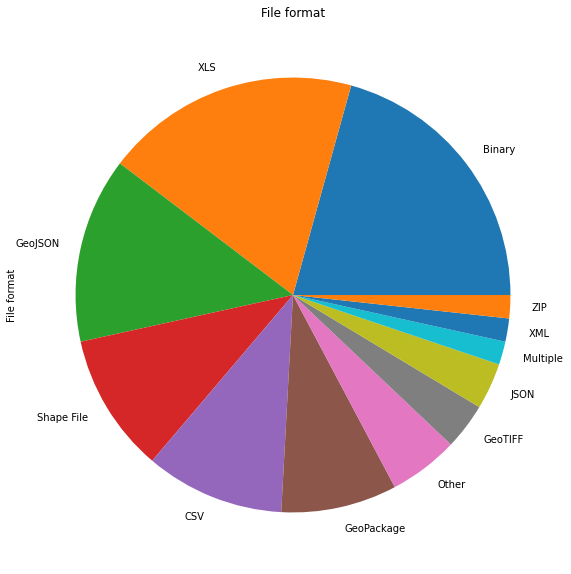
\includegraphics[width=1.0\columnwidth]{figures/foss4g-survey-data.png}
	\caption{eMOTIONAL Cities data formats allocation}
\label{fig:survey-results}
\end{center}
\end{figure}

When surveyed about the purpose of these data, the majority of the researchers in the project mentioned interactive mapping and analysis as their main use cases ~\cite{simoes2021}. With this background in mind, we have selected a set of OGC standards that are best suited to accommodate the project assets in an SDI. In Table~\ref{tab:apis}, we list the selected standards considering the legacy OGC W*s, and their translation to OGC APIs. At the very least, we need to be able to provide access to vector attributes and geometry and provide an interface for web mapping. All datasets should be discovered and accessed through their metadata.

\begin{table}[ht]
    \centering
    \begin{tabular}{|p{0.20\linewidth} | p{0.20\linewidth} | p{0.45\linewidth}|}\hline
      OGC W*s  & OGC API& Description \\\hline
      WFS & Features & Provides access to feature data.\\
      WMTS & Tiles & Provides access to pre-rendered tiles
of geospatial information.\\
      CSW & Records & Provides discovery and access to
metadata about geospatial resources. \\\hline
    \end{tabular}
    \caption{Comparison of OGC API over OGC Web Service standards}
    \label{tab:apis}
\end{table}

%\begin{table}[h]
%	\centering
%		\begin{tabular}{|l|c|c|}\hline
%			OGC W*s&OGCAPI&Accesses\\\hline
%			 WFS&Features&Feature data\\
%			 WMTS&Tiles&Pre-rendered tiles\\
%			 Left&20&0.8\\
%			 Right&20&0.8\\
%			 Column Width&82&3.2\\
%			 Column Spacing&6&0.25\\\hline
%		\end{tabular}
%	\caption{Margin settings for A4 size page.}
%\label{tab:Margin_settings}
%\end{table}

\subsection{Server-side Architecture}\label{sec:SERVER}

Once we selected the standards for the SDI, we set out to select our software stack from existing server-side implementations of the OGC API standards, which are listed under the relevant OGC API GitHub ~\cite{ogcapifeaturesimpl2022,ogcapitilesimpl2022,ogcapirecordsimpl2022}. If available, we would favour choosing OSGeo software, as we would like to benefit from all the advantages of using Free and Open-Source Software (FOSS), including the ability to contribute changes back, if deemed relevant. In the interest of simplicity, we would also prefer software projects that implement more than one of the OGC APIs we selected, and if possible all of them. Currently, there is only one software project that addresses these two requirements: pygeoapi.

pygeoapi is a Python server implementation of the OGC API suite of standards, which “emerged as part of the next generation OGC API efforts in 2018”. It implements a number of OGC APIs, including OGC API - Tiles and OGC API - Features, and it is certified OGC Compliant and an OGC Reference Implementation for OGC API - Features - Part 1: Core 1.0. Rather than being a facade for existing W*s implementations, pygeoapi implements all the OGC APIs from scratch, leveraging all the benefits of modern web practices. For instance, it makes use of HTTP verbs (e.g.: GET/PUT/POST/DELETE) and codes (e.g.: 200, 201, 400, etc) and relies on content negotiation to retrieve the relevant media types. It also adopts JSON (JavaScript Object Notation) encodings, which is very popular among web developers and a first-class citizen in RESTfull (REST- REpresentational State Transfer) web services ~\cite{pygeoapi2019}.

According to the pygeoapi documentation ~\cite{pygeoapiproviders2022}, several data providers are supported for publishing vector data as OGC API - features (see Figure~\ref{fig:pygeoapi-providers}). ElasticSearch, along with SensorThingsAPI, is the data provider which provides the full range of functionality, including support for DateTime, which is an important aspect of neuroscience data.

\begin{figure}[ht!]
\begin{center}
		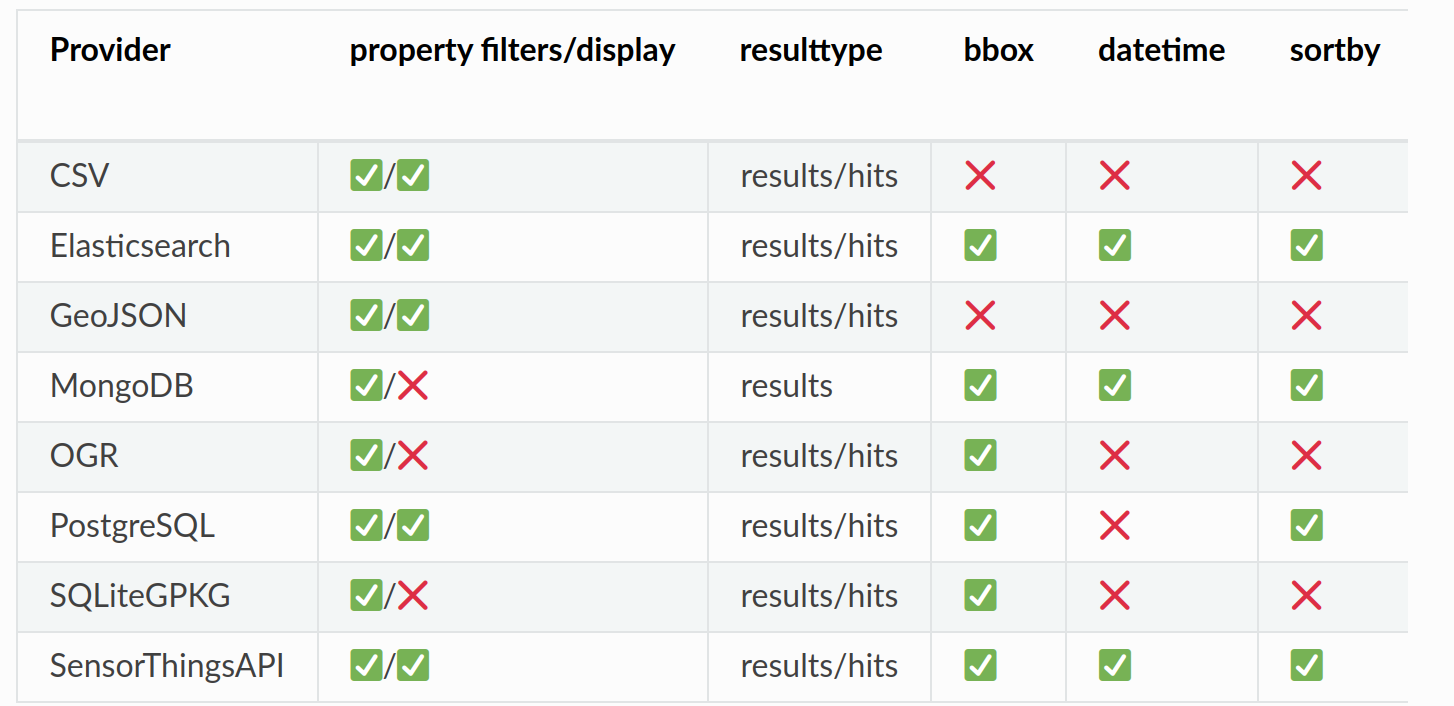
\includegraphics[width=1.0\columnwidth]{figures/pygeoapi-data-providers.png}
	\caption{pygeoapi data providers and functionalities}
\label{fig:pygeoapi-providers}
\end{center}
\end{figure}

ElasticSearch is a search engine, dual-licensed under the source-available Server Side Public Licence and the Elastic licence ~\cite{elasticlicence2022}. It is part of the ELK stack, which includes Logstash, a server‑side data processing pipeline that ingests data from multiple sources simultaneously, transforms it, and then sends it to ElasticSearch and Kibana, a tool to visualise ElasticSearch data with maps, charts and graphs ~\cite{elkstack2022}. By adopting ElasticSearch as a vector data provider for pygeoapi, we can also leverage the complete ELK stack, to ingest and visualise our data assets.

The architecture of the eMOTIONAL Cities SDI is described in Figure~\ref{fig:sdi-arch} and Figure~\ref{fig:docker-compose} of the APPENDIX. Data and metadata are ingested from GeoJSON files in a data lake, and published as OGC API - Features, OGC API - Records and OGC API - Tiles.

\begin{figure}[ht!]
\begin{center}
		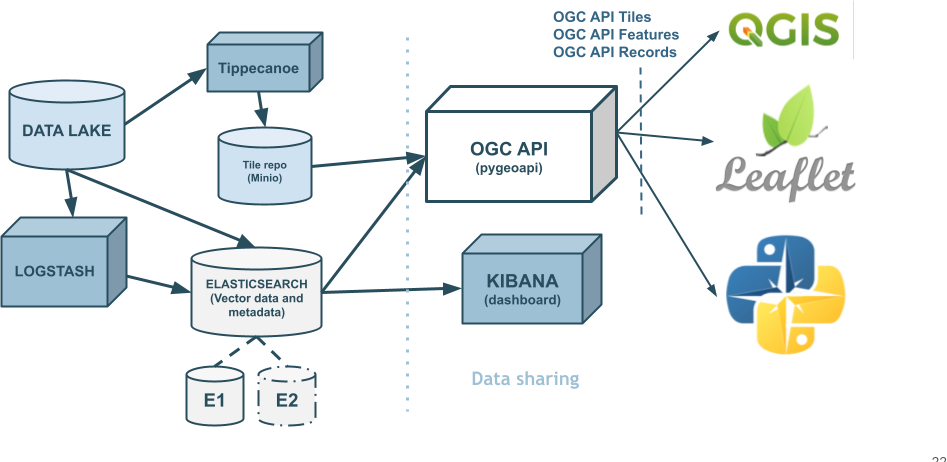
\includegraphics[width=1.0\columnwidth]{figures/sdi-arch.png}
	\caption{eMOTIONAL Cities SDI Architecture}
\label{fig:sdi-arch}
\end{center}
\end{figure}

Tippecanoe ~\cite{tippecanoe2022}, is used to generate vector tiles, which are then served in a Minio bucket ~\cite{minio2022}. MinIO is a High-Performance Object Storage released under a GPL3.0 License. Its API is compatible with the Amazon S3 cloud storage service, which makes it a very good alternative to store large datasets in an unstructured manner, for fast access.

In order to ease the deployment of the SDI and to increase the reproducibility of this research, the software stack was virtualized into a set of docker containers, which are orchestrated using docker-compose (TODO: CITE). The virtualized architecture, described in the diagram below, is published on GitHub, under a GPL License (https://github.com/emotional-cities/openapi-sdi). This stack was deployed at this endpoint, where you can browse through some preliminary datasets from the project: https://emotional.byteroad.net/

\subsection{Clients}\label{sec:CLIENTS}

The availability of client implementations of the selected standards, is a critical aspect of the usefulness of an SDI. While we don’t have software to consume data published under the OGCA API standards, we cannot expect a serious uptake from the users. Our mission in this project does not end with publishing data using the selected standards. We want to make sure that the researchers are able to integrate these data in their workflows, either by using their usual tools, or by using new tools which we should be able to recommend and provide training for. As in the case of server-side implementations, we referred to the GitHub pages of the standards, in order to identify existing client-side implementations of the selected OGC API standards.

OGC API - Features already features eight client implementations, including desktop applications, libraries and JavaScript APIs (TODO: CITE). It is supported in well-known OSGeo projects such as GDAL or QGIS (see Figure~\ref{fig:qgis-oaf}). In addition, as pygeoapi publishes data in GeoJSON, it is compatible with all clients which are capable of consuming GeoJSON.

\begin{figure}[ht!]
\begin{center}
		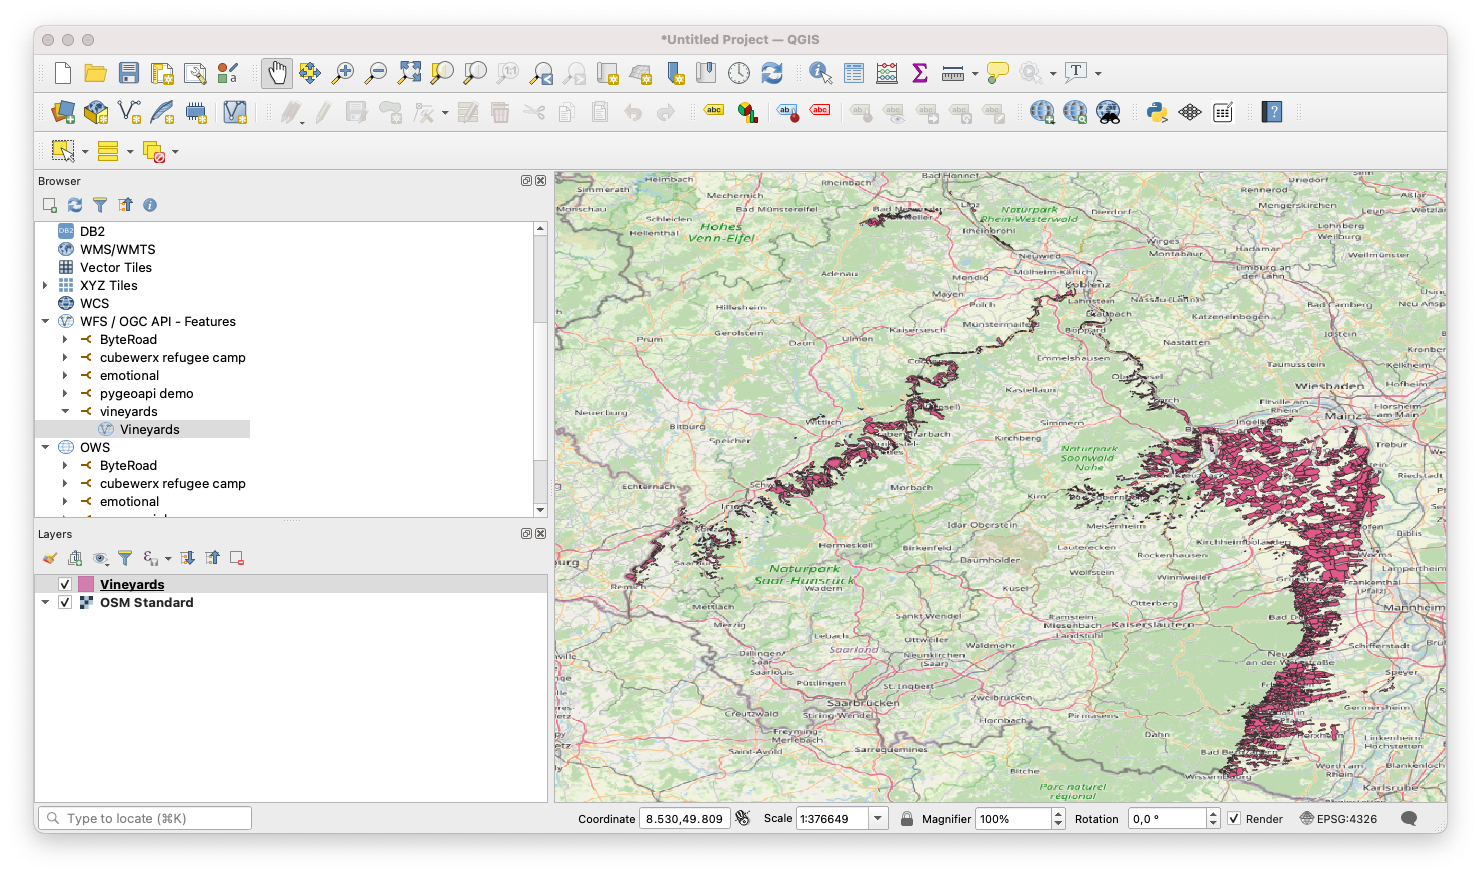
\includegraphics[width=1.0\columnwidth]{figures/qgis-oaf.png}
	\caption{TODO: UPDATE CAPTION.}
\label{fig:qgis-oaf}
\end{center}
\end{figure}

The support to OGC API - Tiles was merged into the main branch of OpenLayers, in September 2021 (https://github.com/openlayers/openlayers/pull/10963). On this repository (TODO CITE), we prototyped a web map consuming vector tiles from OGC API - Tiles, using OpenLayers (see Figure~\ref{fig:ol-oat}).

\begin{figure}[ht!]
\begin{center}
		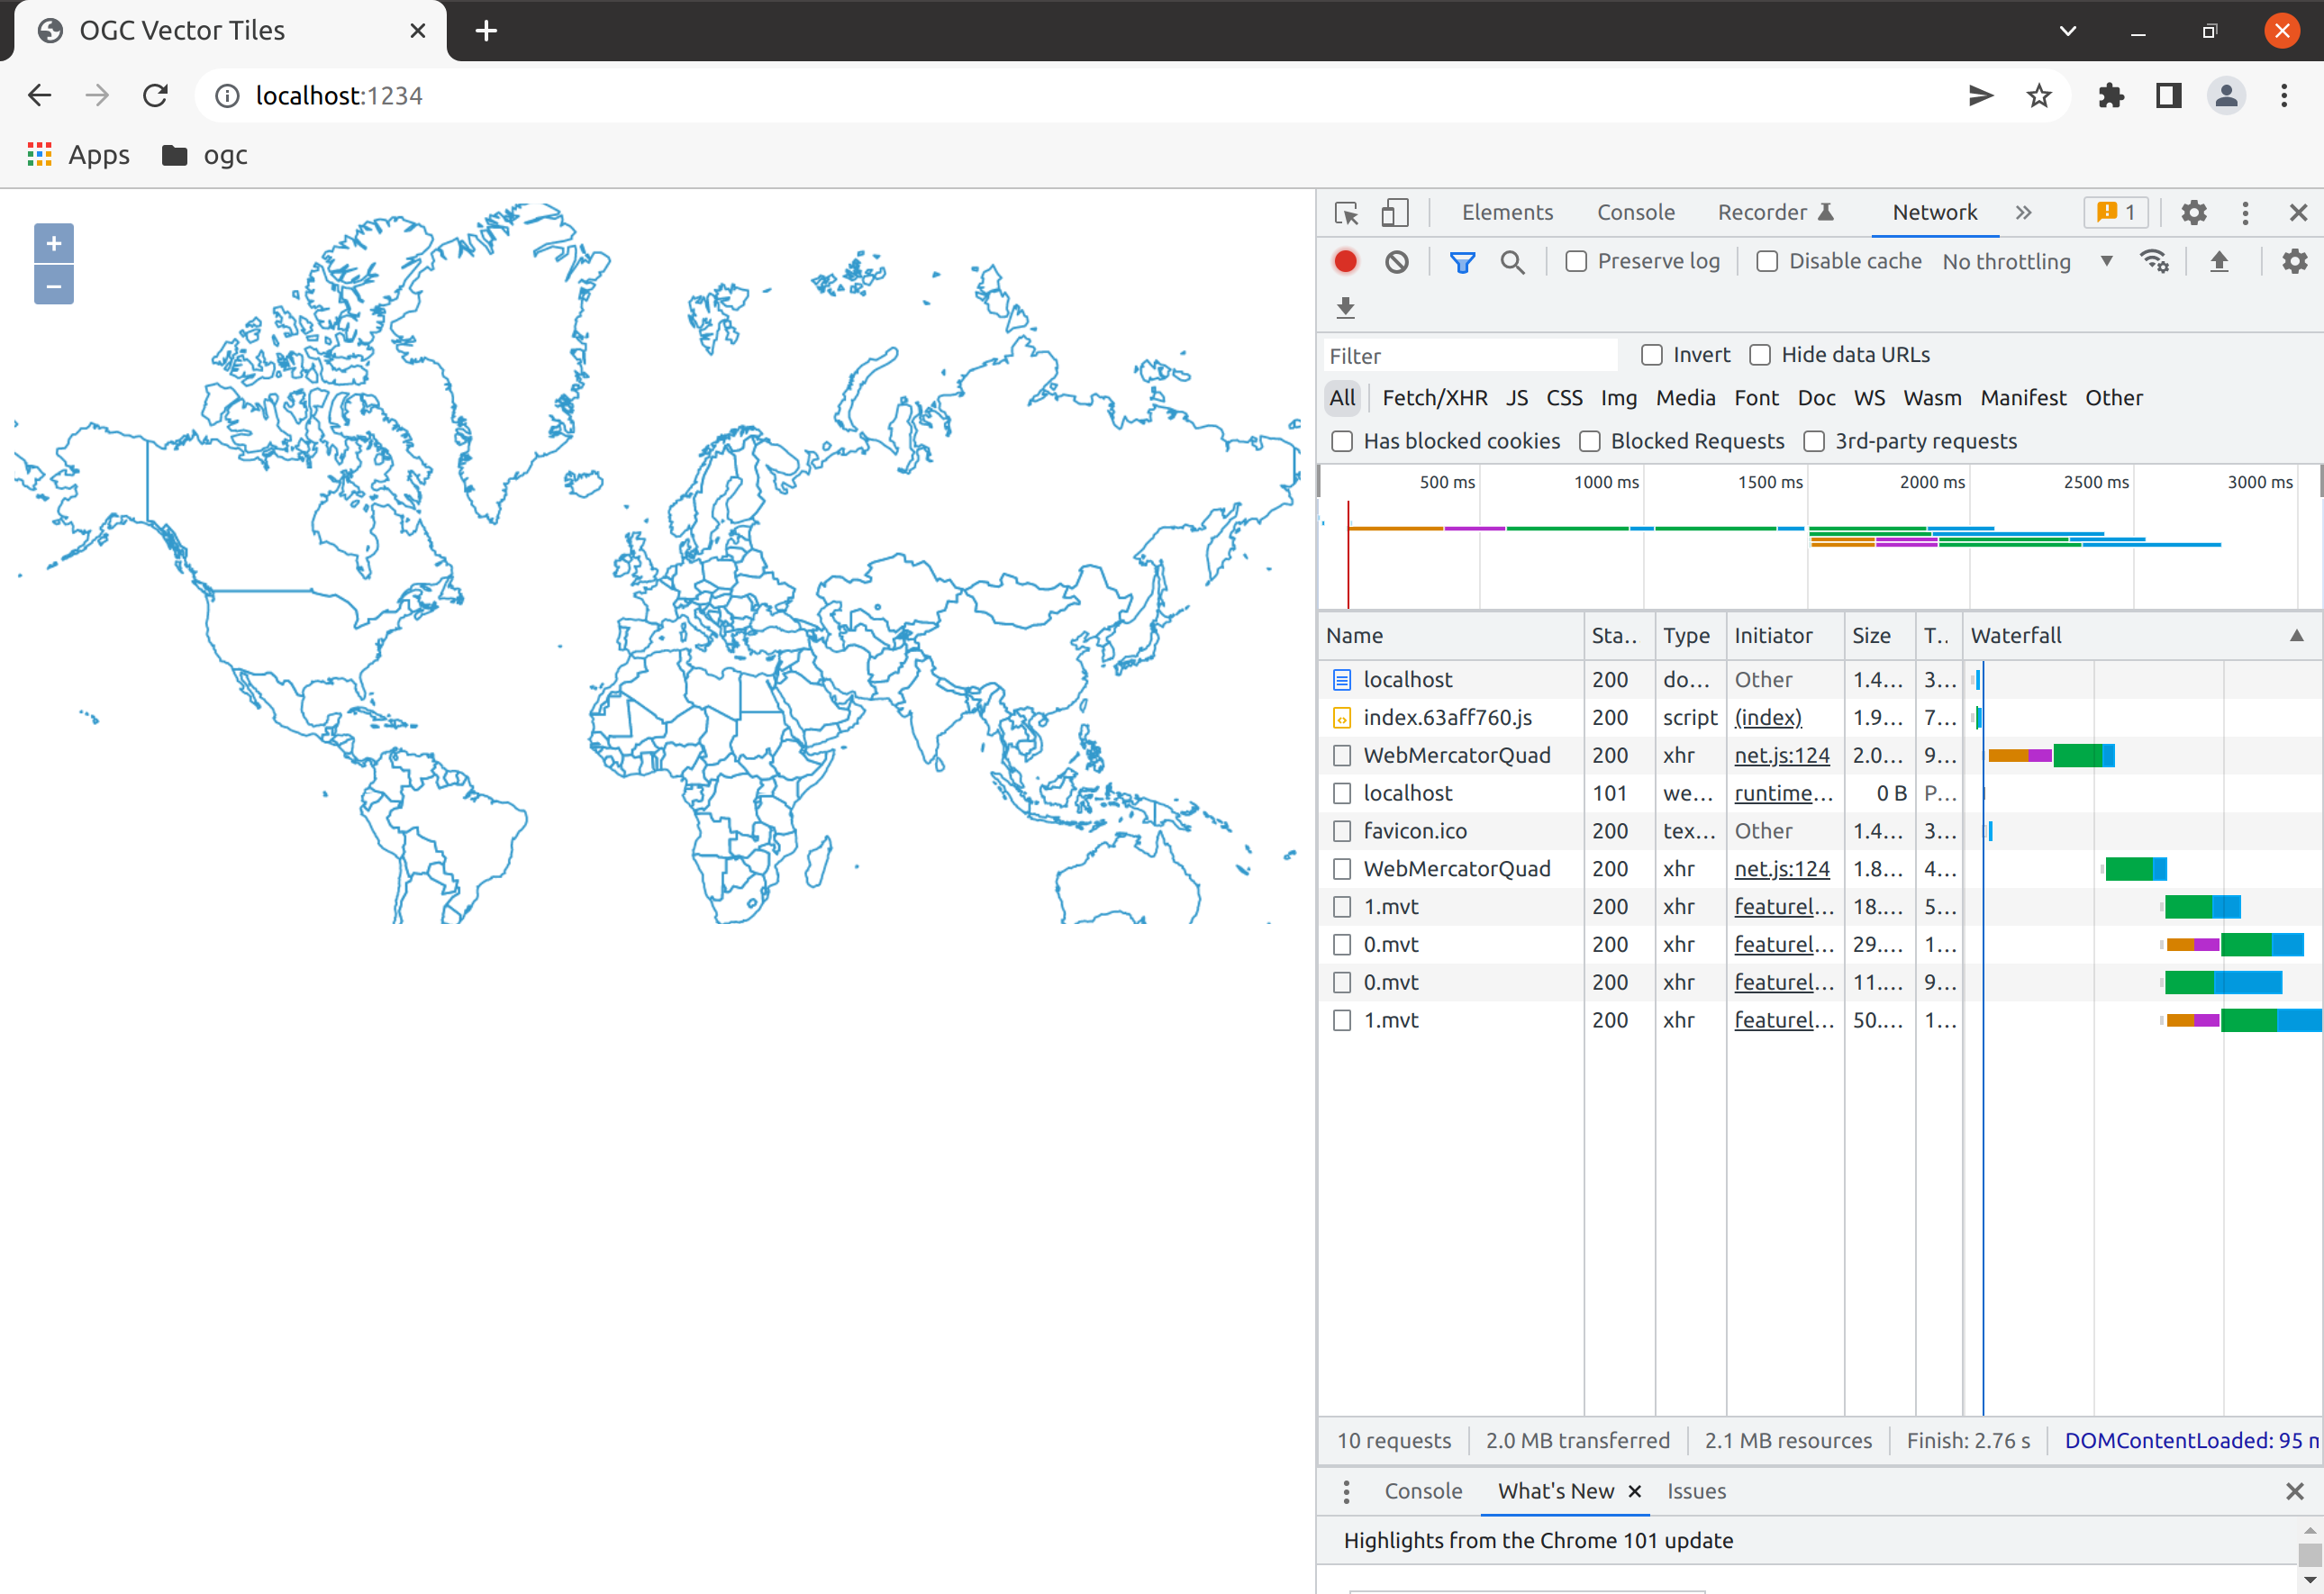
\includegraphics[width=1.0\columnwidth]{figures/ol-oat.png}
	\caption{TODO: UPDATE CAPTION.}
\label{fig:ol-oat}
\end{center}
\end{figure}

Although in the eMOTIONAL Cities SDI we are focused on vector tiles, it is worth mentioning that during the March 2022 Joint OGC-OSGeo-ASF code sprint (TODO Cite), a plugin for Leaflet which adds support for map tiles was prototyped (https://github.com/openlayers/openlayers/pull/10963). 

We provide some considerations about clients for OGC API Records, in section~\ref{sec:METADATA}.

\subsection{The legacy stack}\label{sec:LEGACY}

During the steps of collecting the requirements for the SDI of eMOTIONAL Cities, no participant has explicitly expressed the need to keep or share data following a specific standard. In neuroscience research is, in general, an area where there are not many standards, although the need is recognized (CITE https://link.springer.com/article/10.1007/s12021-021-09557-0), this is no exception to GIS standards. 
For this reason, we have tried to create solutions that rely on emerging technological trends and thus are more likely to stay around in the future. However, researchers from the urban planning domain are often used to work with the legacy W*s, and as we described in section~\ref{sec:CLIENTS}, there are not that many client implementations available, which means that in some cases their preferred tool may not support an OGC API, yet. As a compromise, we decided to provide a backward compatibility system. This has led us to deploy a legacy stack, composed of mature free and open-source solutions widely used in the GIS domain, along with our OGC API stack.

The legacy stack is built around the free and open-source GeoServer, which implements industry-standard OGC protocols such as Web Feature Service (WFS), Web Map Service (WMS), and Web Coverage Service (WCS). Additional formats and publication options are available as extensions including Web Processing Service (WPS), and Web Map Tile Service (WMTS). (CITE https://geoserver.org/). The architecture of this solution is described in Figure~\ref{fig:sdi-legacy-arch} and in Figure~\ref{fig:docker-compose-legacy} of the APPENDIX.

\begin{figure}[ht!]
\begin{center}
		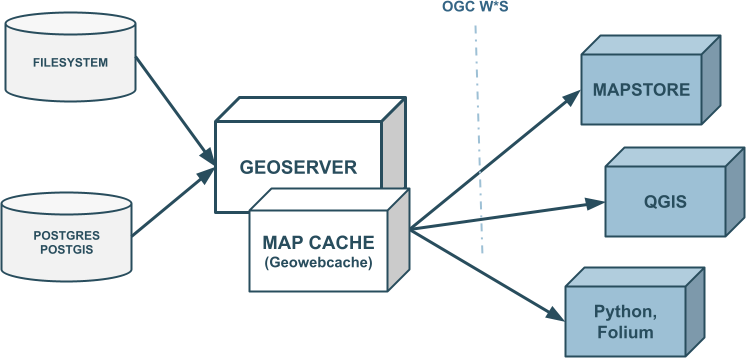
\includegraphics[width=1.0\columnwidth]{figures/sdi-legacy-arch.png}
	\caption{TODO: UPDATE CAPTION.}
\label{fig:sdi-legacy-arch}
\end{center}
\end{figure}

GeoServer can be configured to collect data from different sources, like filesystems and DBs (spatial and non). 
As part of the project, GeoServer will exclusively share data, which will be gathered in the Data Lake, the same used in the OGC API stack, and ingested in GeoServer’s stores by suitably configured data pipelines. A diagram with the server side architecture of this stack is shown below.
Data from GeoServer can be easly consumed by a wide range of GIS clients, including the MapStore, an highly modular Open Source WebGIS framework, included in the EC’s SDI (https://mapstore.readthedocs.io/en/latest/).

\subsection{Metadata}\label{sec:METADATA}

In a project built around FAIR principles, metadata leads a primary role. Metadata allows the description of the datasets exposed by the other components of the SDI, making the data searchable and accessible. Using metadata to describe resources enables its understanding by humans as well as machines. The literature is rich on the subject, and it is not an exaggeration to consider an SDI complete only when it is provided with a catalogue of its data. (CITE http://aims.fao.org/news/fair-principles-digital-objects-role-metadata)
The reference standard for catalogues of GIS records is the OGC CSW. In CSW, metadata records are XML documents served over HTTP. CSW is a profile of the OGC Catalog Service specification (CITE https://www.ogc.org/standards/cat).
OGC API - Records (from now OARec) specification has been developed with the same objective as CSW, but built with the characteristics of an OGC API.
Unlike CSW, which exposes records as XML documents, OARec can expose records in different formats, although the JSON format remains an essential requirement (CITE ).
According to (Cite draft 20 004) there are a number of ways that records can be deployed as a "collection of records" or a catalogue.
\begin{itemize}
\item {Crawlable catalogue: To implement a catalogue where records are stored as individual files in one or more web-accessible locations and can be crawled by simply following hypermedia controls.1}
\item {Searchable catalogue: To implement a catalogue where records are stored in some backend database and are accessed through an access/search API.1}
\item {Local resources catalogue: To implement a local resource catalogue at an OGC API resources endpoint.1}
\end{itemize}
(CITE )
Deciding which record catalogue to use for EC was not an easy choice, because metadata is the single entry point of an SDI, and thus it does not make sense to have multiple deployments, using legacy and modern standards. Therefore, it was decided to use the OGC API option, since it makes no sense to present an entry point that does have the characteristics and benefits that we favour adopting in the other solutions.
The exploratory nature of the project allows for this choice, but the impossibility of recommending this choice in other fields, such as public administrations and governments, must however be mentioned. First of all, the fact that the standard is still in draft, although its maturity must be recognized. Not least importantly, given the fundamental role of metadata in an SDI, is the fact that the standard is not yet stable enough to be covered under national and international directives, such as INSPIRE, for which OGC CSW still remains a safer choice (CITE ).
Having said that, the promising uptake of the standard, which even in an early stage of development, already features server-side implementations must be acknowledged. Free and Open Source solutions, such as pygeoapi, allow users to have an implementation of OARec aligned with advances in standards, which is perfectly usable in a real SDI (CITE ).

On the client-side, the OGC API - Records searchable catalogue is supported natively in QGIS, through the Metasearch core plugin (TODO: Cite). Figure~\ref{fig:qgis-rec} shows a screenshot of this plugin, which allows users to browse through the records of OGC API - Records catalogues, view the metadata and pull the associated data. This tool does not provide however, an interface for the authoring of metadata. 

\begin{figure}[ht!]
\begin{center}
		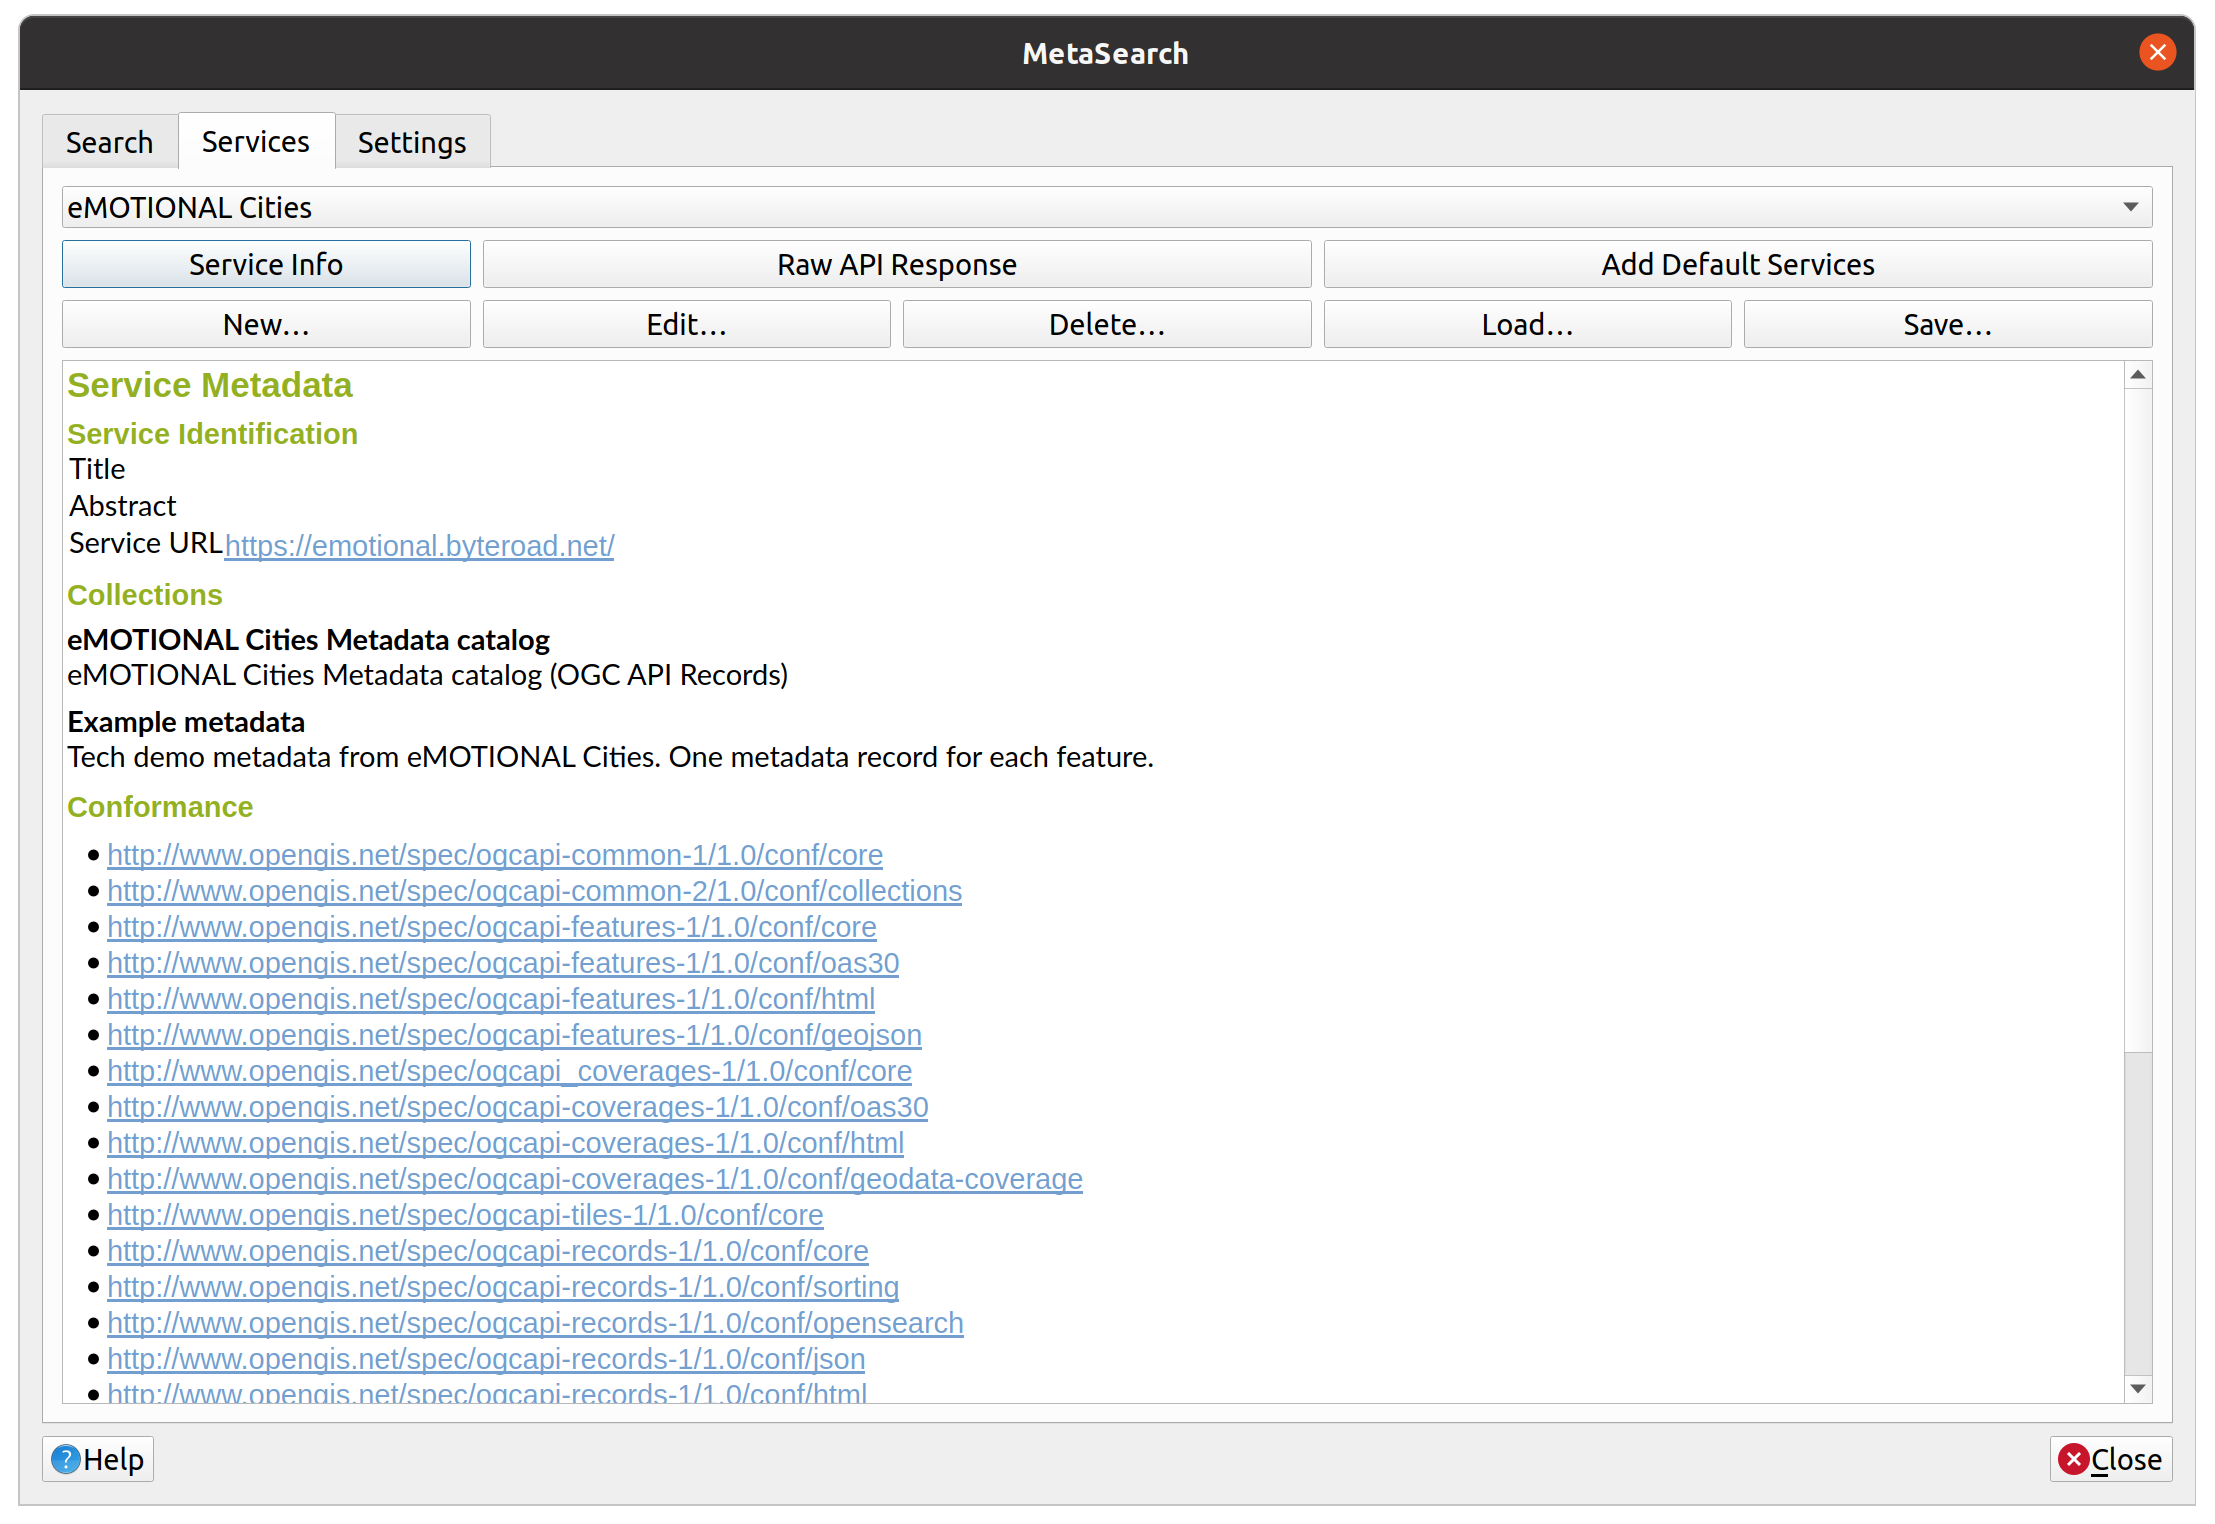
\includegraphics[width=1.0\columnwidth]{figures/ec-records.png}
	\caption{TODO: UPDATE CAPTION.}
\label{fig:qgis-rec}
\end{center}
\end{figure}

We also did not find any web application, which enabled browsing OGC API - records on the web, apart from the compatible STAC Vue browser, which is restricted to crawlable catalogues  (https://github.com/radiantearth/stac-browser). A screenshot of this application is shown on Figure~\ref{fig:stac-browser}. 

\begin{figure}[ht!]
\begin{center}
		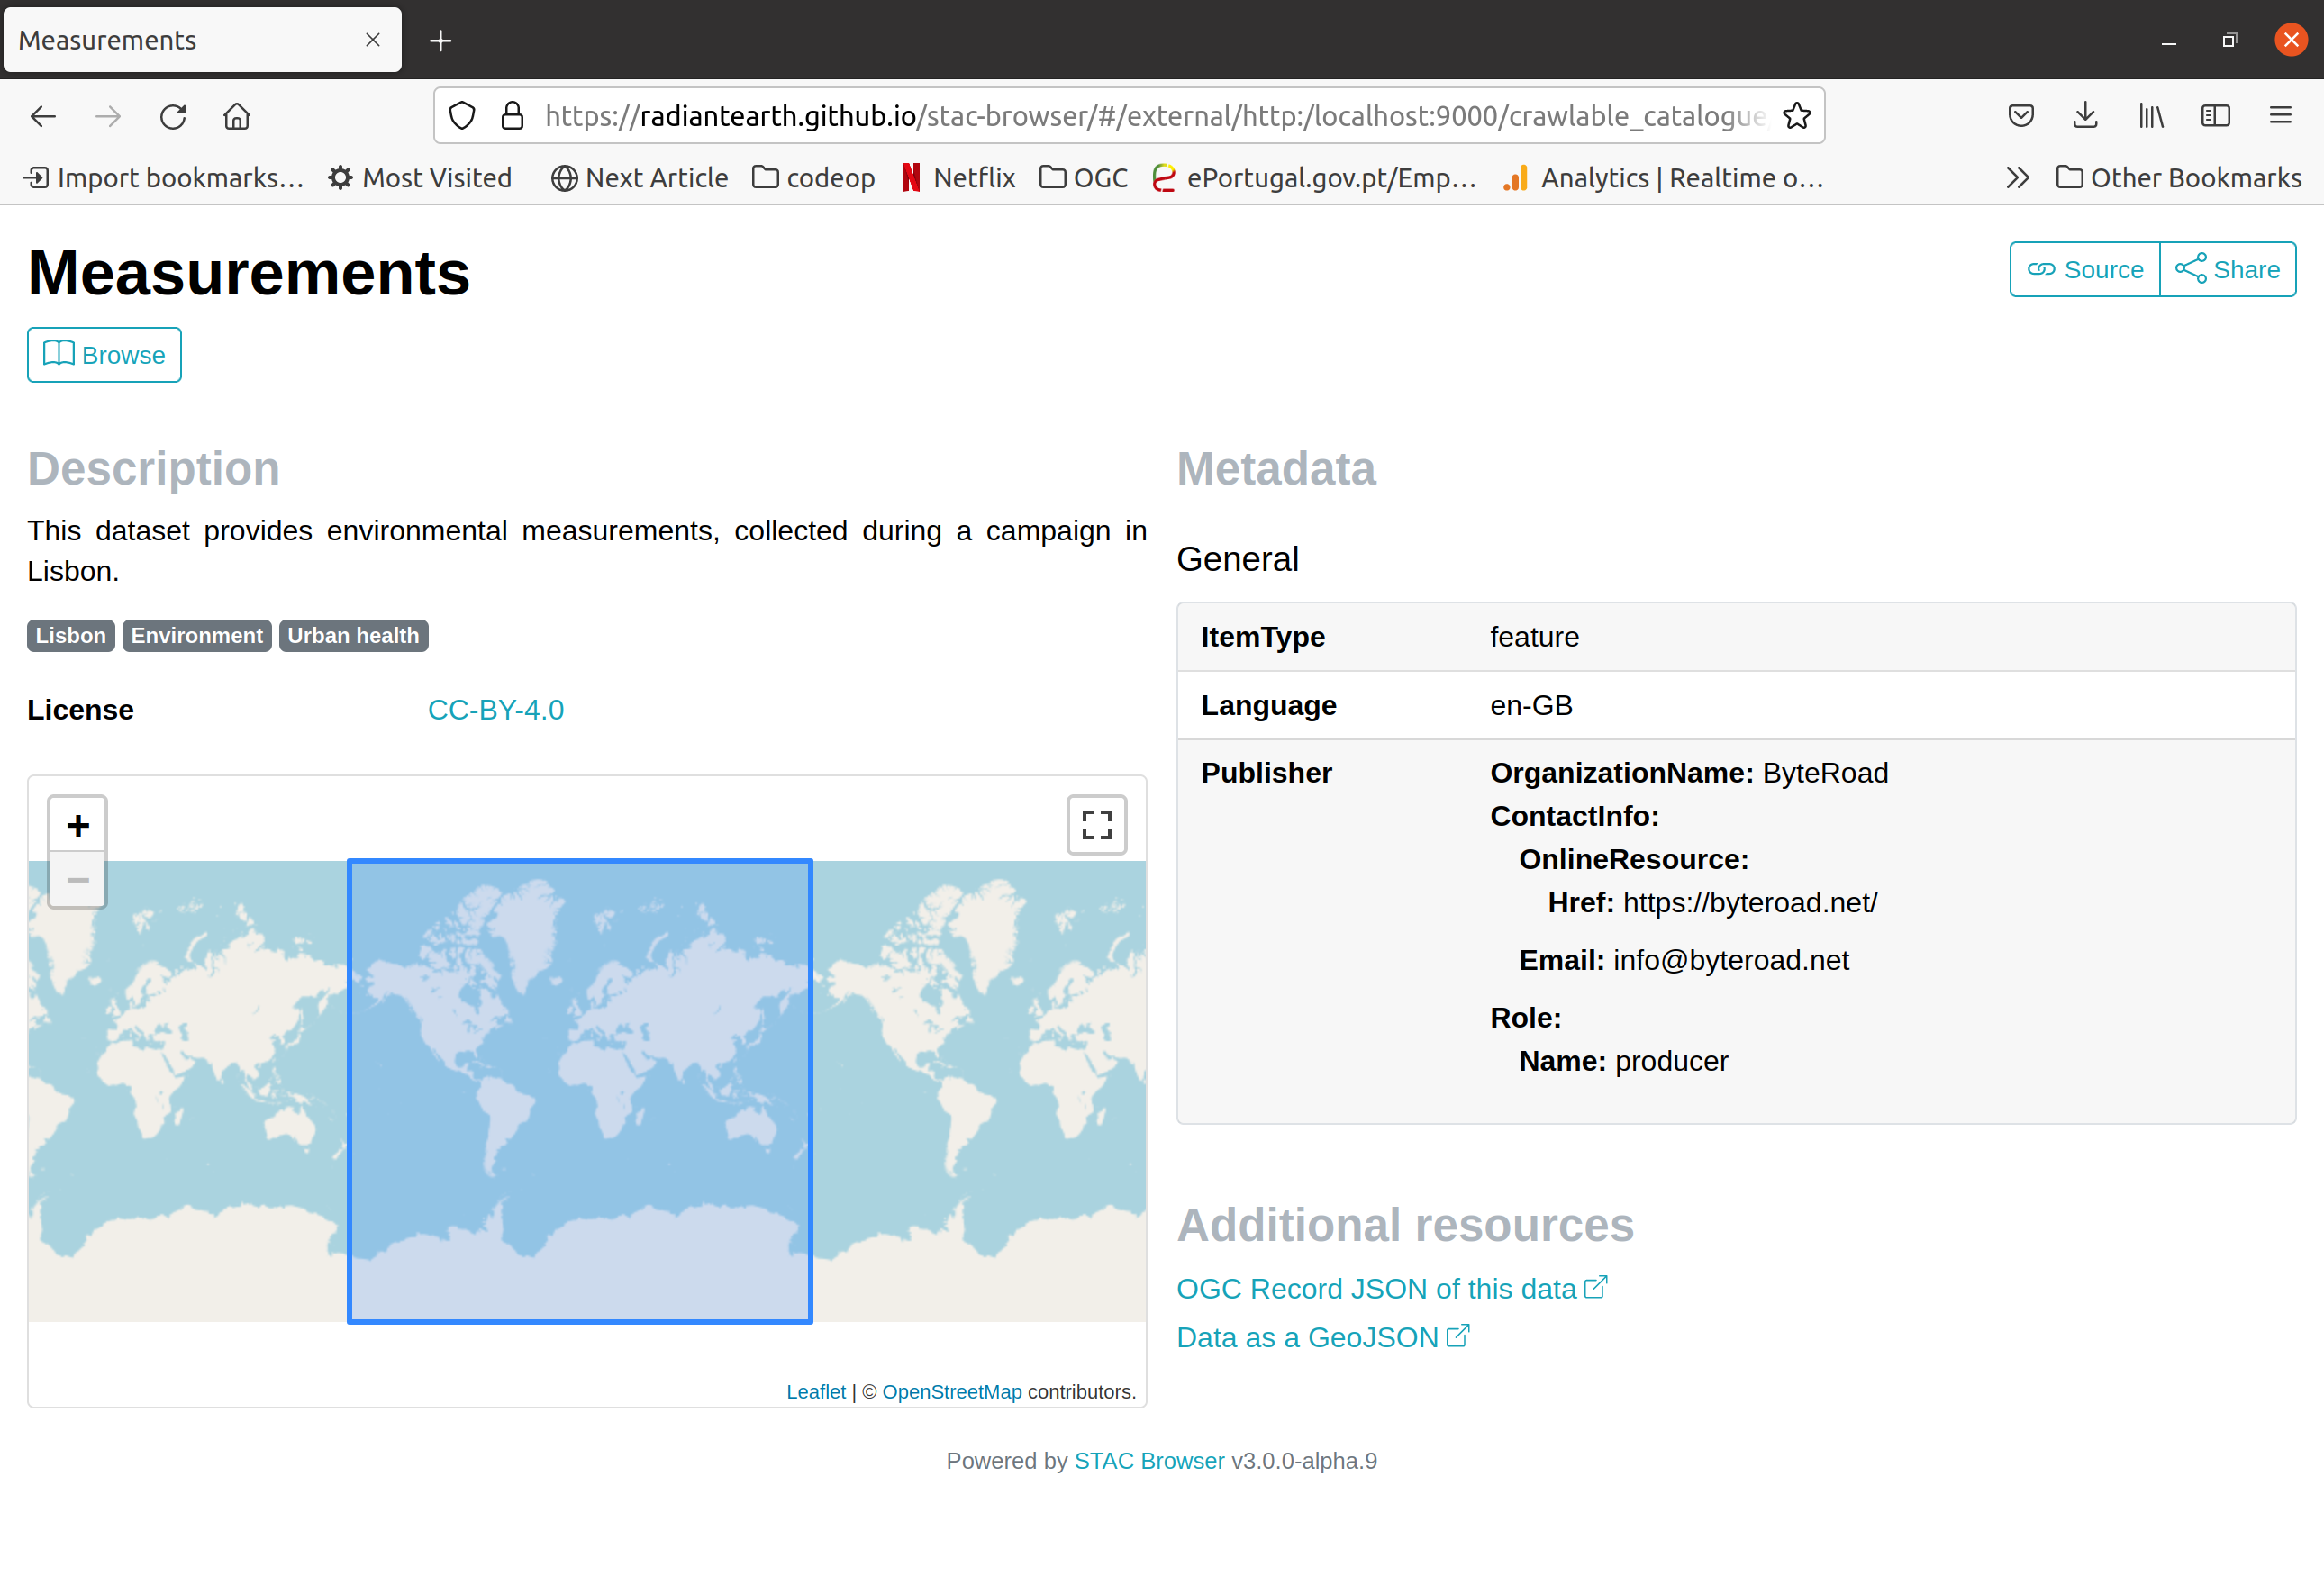
\includegraphics[width=1.0\columnwidth]{figures/crawlable-catalogue-stac.png}
	\caption{TODO: UPDATE CAPTION.}
\label{fig:stac-browser}
\end{center}
\end{figure}

This has led us to develop a metadata browser, A-gis-full-of-records, using React Framework (CITE https://reactjs.org/) and Leaflet (CITE https://leafletjs.com/). The tool, shown on Figure~\ref{fig:metadata-browser}, is still under development, but it’s a good demonstration of the developer friendliness of OGC API.

\begin{figure}[ht!]
\begin{center}
		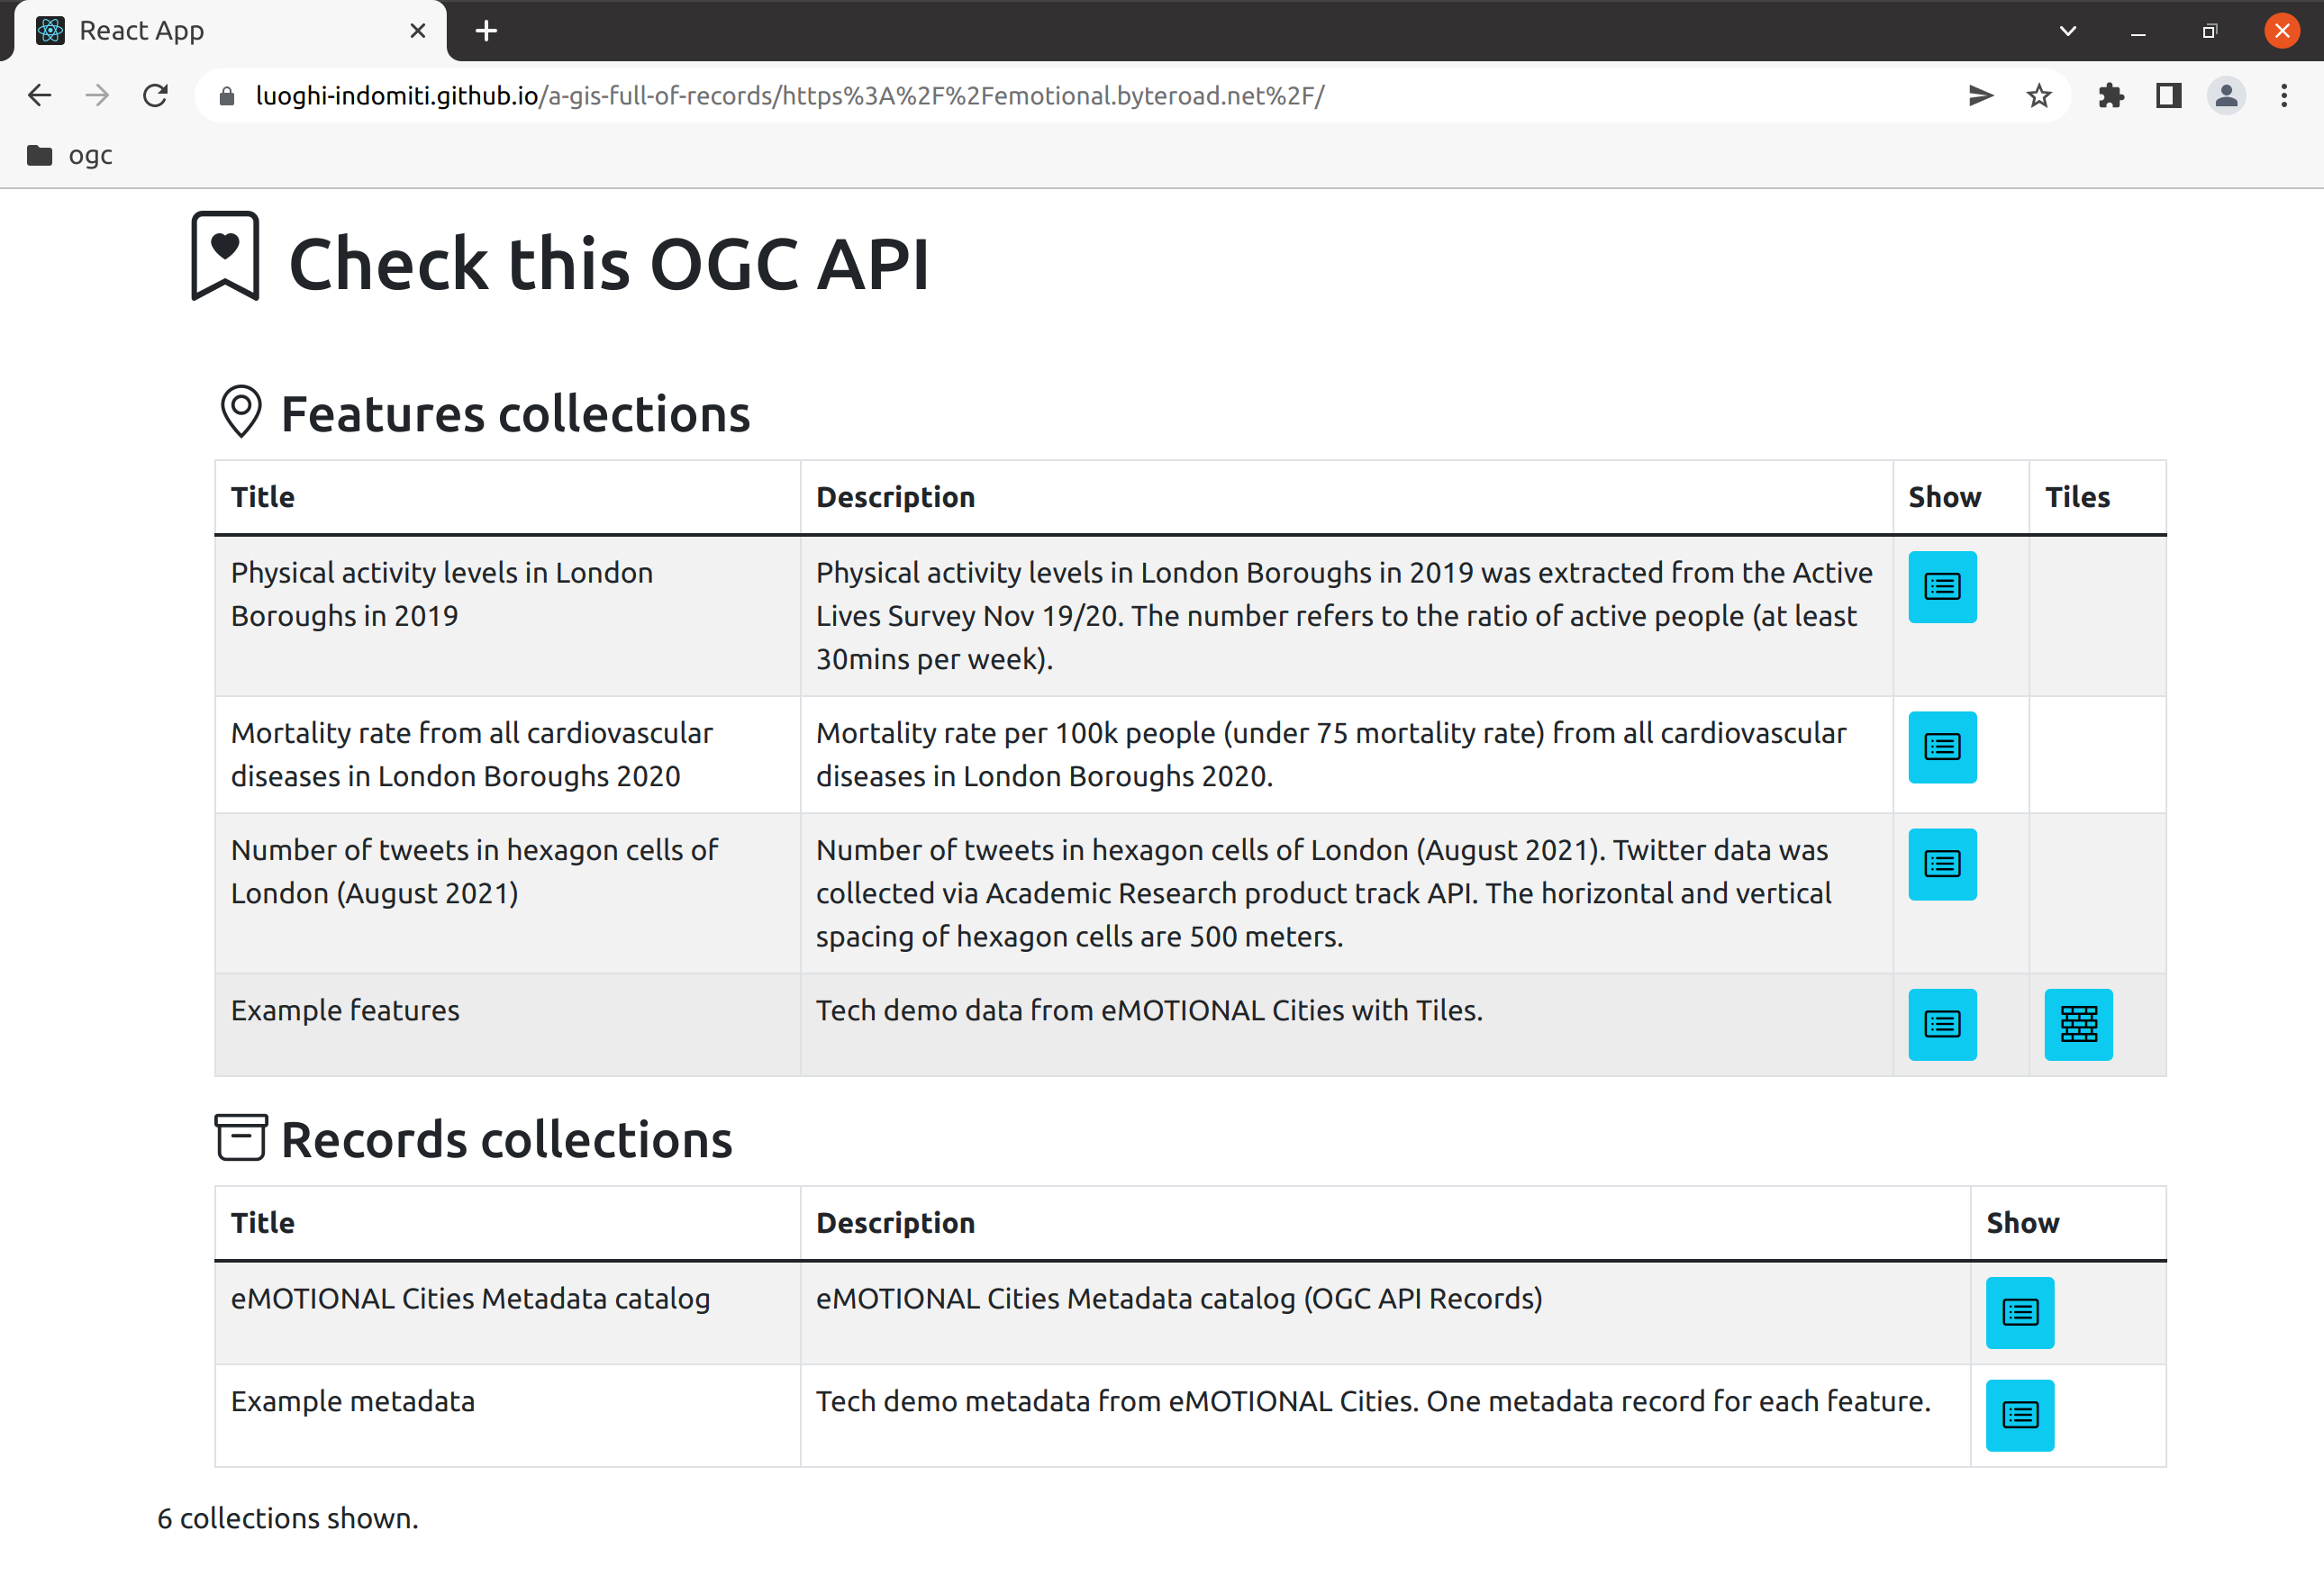
\includegraphics[width=1.0\columnwidth]{figures/metadata-browser.png}
	\caption{TODO: UPDATE CAPTION.}
\label{fig:metadata-browser}
\end{center}
\end{figure}

\section{Discussion and Conclusions}\label{CONCLUSIONS}

The OGC APIs promise exciting features for modern SDIs. Although (at least some of them are) still at an early stage, there is an active development taking place in code sprints and GitHub repositories, inclusive of the developer community and welcomes feedback.
Similarly to what happens with OSGeo projects, hopefully, this trend will lead to high-quality specs with increased ownership from the developer community. 
We were surprised to see that it is already possible to implement a server-side architecture for an SDI entirely based on OGC APIs and OSGeo software. pygeoapi proved to be a sound solution for implementing multiple OGC API standards. It is very easy to install, especially using the official docker image (TODO cite reference), and is very flexible through its modular architecture, which relies on plugins for multiple data providers. Although the project is under active development, since it is free and open-source, we were able to contribute to its development.

However, in terms of clients, there are still few implementations, and widely used products by the GIS community (e.g. Leaflet, MapStore, Kibana) still lack native support to the OGC APIs, along with their support to legacy W* services. 

This has led us to deploy a stack for the legacy W*s to enable the GIS researchers from the eMOTIONAL Cities project to access the project data assets using their usual tools. We believe this type of hybrid solution will work for many use cases, such as public services or research projects, where there are GIS experts, trained in legacy W*s services but with little knowledge about the OGC APIs. However, it should be mentioned that even in those cases, it will be easier to onboard a web developer with no knowledge of GIS to use the OGC APIs than to use the legacy stack.

Although we have described many advantages of the OGC APIs, we believe there will be no massive uptake until enough client implementations are available and users are trained to use them. We are committed to these two fronts and have already delivered training in using clients during the OGC code sprints (TODO CIte) and started our client developments. We hope these efforts, within the scope of the four year eMOTIONAL Cities project, will contribute to the development of the OGC APIs and, not least significantly, towards their visibility, within the GIS community and the broader developer community. 




%Mark footnotes in the text with a number (1); use consecutive numbers for following footnotes. Place footnotes at the bottom of the page, separated from the text above it by a horizontal line.


%\subsection{Illustrations and Tables}\label{sec:Illustrations and Tables}

%\subsubsection{Placement:}\label{sec:Placement}

%Figures must be placed in the appropriate location in the document, 
%as close as practicable to the reference of the figure in the text. 
%While figures and tables are usually aligned horizontally on the page, 
%large figures and tables sometimes need to be turned on their sides. 
%If you must turn a figure or table sideways, please be sure that the 
%top is always on the left-hand side of the page.


%\subsubsection{Captions:}\label{sec:Captions}

%All captions should be typed in upper and lower case letters, 
%centred directly beneath the illustration. Use single spacing if they 
%use more than one line. All captions are to be numbered consecutively, 
%e.g. Figure~1, Figure~2, Figure~3, ..  and Table~1, Table~2, Table~3, ...

% KAO: Remove spacing before label: can cause reference to be wrong

% KAO: Inter-sentence spacing
%If your article contains any copyrighted illustrations or imagery, 
%please include a statement of copyright such as: \copyright~SPOT Image Copyright 20xx 
%(fill in year), CNES\@. It is the author's responsibility to obtain any necessary 
%copyright permission. After publication, your article is distributed under %\underline{the Creative 
%Commons Unported License} and you retain the copyright.


% % KAO: Non-breaking space

\section*{ACKNOWLEDGEMENTS}\label{ACKNOWLEDGEMENTS}
Acknowledgements of support for the project/paper/author are masked, in order to not violate the anonymity of the submitted paper. 

%\section*{REFERENCES}\label{REFERENCES}
{
	\begin{spacing}{1.17}
		\normalsize
		\bibliography{ISPRSguidelines_authors} % Include your own bibliography (*.bib), style is given in isprs.cls
	\end{spacing}
}

\pagebreak
\onecolumn

\section*{APPENDIX}\label{APPENDIX}

\begin{figure}[ht!]
\begin{center}
		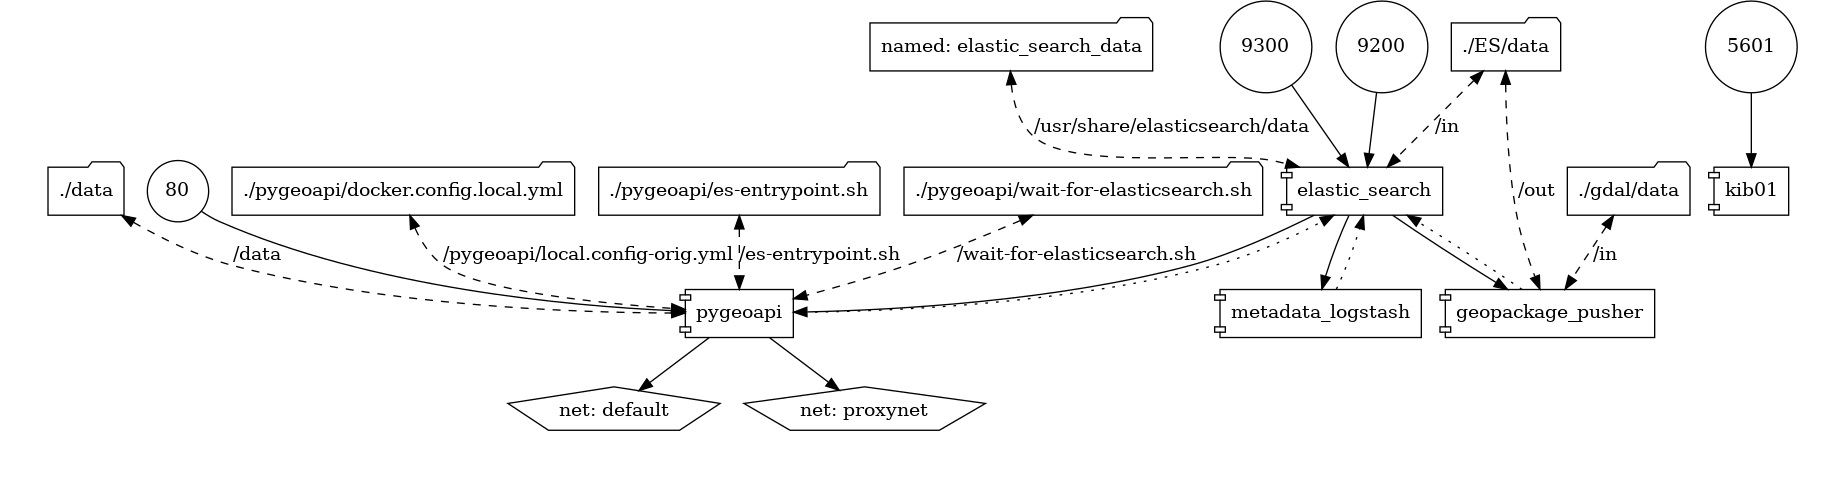
\includegraphics[width=1.0\columnwidth]{figures/docker-compose-all.png}
	\caption{TODO: UPDATE CAPTION.}
\label{fig:docker-compose}
\end{center}
\end{figure}

\begin{figure}[ht!]
\begin{center}
		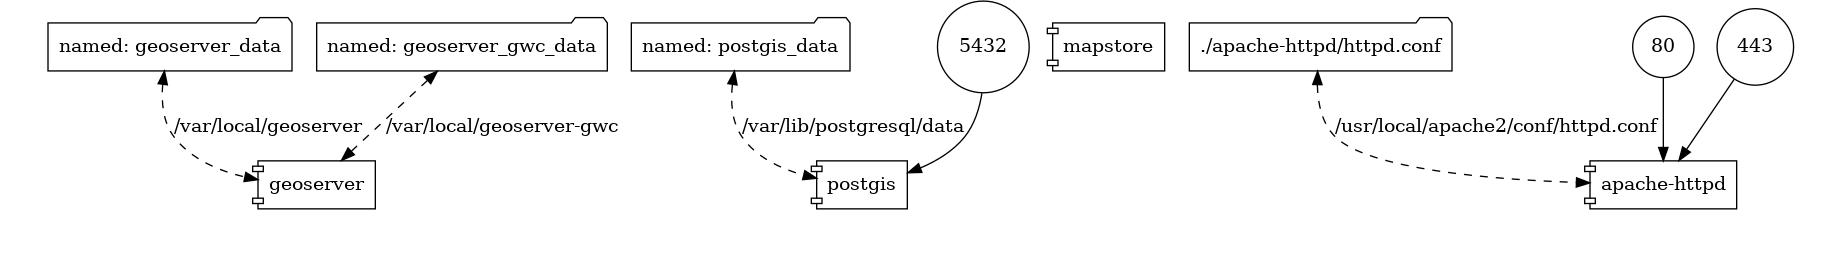
\includegraphics[width=1.0\columnwidth]{figures/docker-compose-legacy.png}
	\caption{TODO: UPDATE CAPTION.}
\label{fig:docker-compose-legacy}
\end{center}
\end{figure}


\end{document}
